% Die Beamer-Klasse unterstützt folgende Optionen, die von
% besonderem Interesse sind (alle Standardoptionen werden
% ebenfalls unterstützt; siehe beamer-Basisdokumentation):
% 
%%%%%%%%%%%%%%%%%%%%%%%%%%%%%%%%%%%%%%%%%%%%%%%%%%%%%%%%%%%%%%%
% aspectratio: Seitenverhältnis des resultierenden Dokuments
% (Achtung: Aufgrund der Designvorgaben ergeben sich unterschiedliche
% Größen der effektiv nutzbaren Textblöcke)
%
% Standardeinstellung: 'aspectratio=43'
%
% Mögliche Einstellungen:
% 'aspectratio=43'   (4:3)
% 'aspectratio=169'  (16:9)
% 'aspectratio=1610' (16:10)
% 
%%%%%%%%%%%%%%%%%%%%%%%%%%%%%%%%%%%%%%%%%%%%%%%%%%%%%%%%%%%%%%%
% fontsize: Basisschriftgröße (Größen für Überschriften etc. werden
% aus dieser Basis automatisch abgeleitet)
%
% Standardeinstellung: '22pt' (entspricht den Design-Vorgaben; sehr groß!)
%
% Mögliche Einstellungen:
% '8pt', '9pt', '10pt', '11pt', '12pt', '14pt', '16pt',
% '17pt','20pt','22pt', '24pt', '26pt', '28pt'


\documentclass[aspectratio=169,16pt]{beamer}

% Der OTHR-Theme unterstützt folgende Optionen:
% 
%%%%%%%%%%%%%%%%%%%%%%%%%%%%%%%%%%%%%%%%%%%%%%%%%%%%%%%%%%%%%%%
% department: (Wahl der Abteilung/Fakultät)
%
% default: 'OTHR'
%
% Mögliche Einstellungen:
% 'FakA', 'FakAM', 'FakB', 'FakBW', 'FakEI', 
% 'FakIM', 'FakM', 'FakS', 'ZWW', 'IPF',
% 'SappZ', 'KNB', 'ReMIC', 'LFD', 'LAS3',
% 'DK0PT', 'LBM', 'LeanLab', 'LFT', 'LFW',
% 'LMP', 'LMS', 'LRT', 'LWS', 'RRRU',
% 'RST', 'CEEC', 'FEM', 'IST'
%%%%%%%%%%%%%%%%%%%%%%%%%%%%%%%%%%%%%%%%%%%%%%%%%%%%%%%%%%%%%%%%%
% headerMode: Aussehen und Inhalt der Kopfleiste
%
% Standardeinstellung: 'full'
%
% Mögliche Einstellungen:
% 'full', 'frametitle', 'frametitleSection'
% 

%%%%%%%%%%%%%%%%%%%%%%%%%%%%%%%%%%%%%%%%%%%%%%%%%%%%%%%%%%%%%%%%%
% Binäre Schalter (können angegeben oder nicht angegeben werden;
% Standardeinstellung: Nicht angegeben)
%
%%%%%%%%%%%%%%%
% navbar: Navigationssymbole anzeigen (Seite vor/zurück, Kapitel vor/zurück etc.)

% pageNumbers: Seitennummerierung

% blackFont: Nur schwarze Schriftfarbe verwenden (ansonsten: Fakultätsfarben)

% frametitleCenter: Titel in der Kopfzeile zentrieren (ansonsten: rechtsbündig)

\usetheme[department=FakIM,pageNumbers]{OTHR}

% Inhaltsspezifische Zusatzpakete laden 
\usepackage[ngerman]{babel}
\usepackage[utf8]{luainputenc}
\usepackage[ngerman]{babel}
\usepackage[utf8]{luainputenc}
\usepackage{filecontents}
\usepackage{subfigure}
\usepackage{numprint}
\usepackage{tikz}
\usepackage{tikzpagenodes}
\usetikzlibrary{calc, shapes, backgrounds, arrows}
\usepackage{ragged2e} 
\usepackage{blindtext}
\usepackage{enumerate}
\usepackage{calc}
\usepackage{graphicx}
\usepackage[absolute,overlay]{textpos}  % in der Präambel
\usepackage{tikz}
\usepackage{algorithm}
\usepackage{algpseudocode}
\usepackage{amsmath}  
\usepackage{listings}
\usetikzlibrary{positioning}
\usepackage{booktabs}
\usepackage{multirow}

\usepackage[most]{tcolorbox}


\begin{document}


\lstdefinestyle{mystyle}{
	language=Python,
	basicstyle=\ttfamily\small,
	keywordstyle=\color{blue},
	commentstyle=\color{gray},
	stringstyle=\color{orange},
	showstringspaces=false,
	breaklines=true,
	frame=singe
}
\renewcommand\lstlistingname{Code}

\lstset{style=mystyle}

\title{Präsentation der Masterarbeit}
\subtitle{On Homotopy of Similar Neural Networks using Non-linear Transformations}
\author{Bettina Zieger}

\begin{textblock*}{5cm}(12cm,0cm)  % Breite, (x,y)-Position in cm
	
\includegraphics[width=0.7\linewidth]{BilderPräsentation/aisec_logo.pdf}
\end{textblock*}
	


\institute{Fakultät Informatik und Mathematik}
\date{24.07.2025}

\begin{filecontents}{\jobname.bib}
@inproceedings{
chan_affine_2024,
title={On Affine Homotopy between Language Encoders},
author={Robin Chan and Reda Boumasmoud and Anej Svete and Yuxin Ren and Qipeng Guo and Zhijing Jin and Shauli Ravfogel and Mrinmaya Sachan and Bernhard Sch{\"o}lkopf and Mennatallah El-Assady and Ryan Cotterell},
booktitle={The Thirty-eighth Annual Conference on Neural Information Processing Systems},
year={2024},
url={https://openreview.net/forum?id=FTpOwIaWUz}
}

\end{filecontents}

% Zitationsstil wählen: amsalpha
\bibliographystyle{plain}

\maketitle
\frame{\tableofcontents \begin{textblock*}{5cm}(12cm,0cm)  % Breite, (x,y)-Position in cm
		
\includegraphics[width=0.7\linewidth]{BilderPräsentation/aisec_logo.pdf}
\end{textblock*}}

\section{Motivation}
\frame{\tableofcontents[currentsection]}
% --- Folie 2: Forschungsfrage ---
\begingroup
\frametitle{Fraunhofer AISEC}
\begin{frame}
	\begin{figure}
		\centering
		\includegraphics[width=0.7\linewidth]{BilderPräsentation/AISEC.png}
		\caption{Fraunhofer-Institut in Garching}
		\label{fig:enter-label}
	\end{figure}
	\vspace{0.2em}
	\begin{itemize}
		\item Fraunhofer-Institut für Angewandte und Integrierte Sicherheit in Garching
		\item Cognitive Security Technologies
		\begin{itemize}
			\item Künstliche Intelligenz und IT-Sicherheit
		\end{itemize}
	\end{itemize}
\end{frame}
\endgroup


\begingroup
\frametitle{Motivation}
\begin{frame}
	\begin{itemize}
		
		\uncover<1->{
			\item[] Neuronale Netze dominieren viele Bereiche:
			\item[]
			{\scriptsize
				\begin{tabular}{@{}p{0.45\textwidth}@{\hspace{1.4em}}p{0.45\textwidth}@{}}
					\hspace{1.4em}
\includegraphics[height=1em]{BilderPräsentation/image.png} Bildverarbeitung &
					
\includegraphics[height=1em]{BilderPräsentation/alert.png} Anomalieerkennung \\
					\hspace{1.4em}
\includegraphics[height=1em]{BilderPräsentation/text.png} Textverarbeitung &
					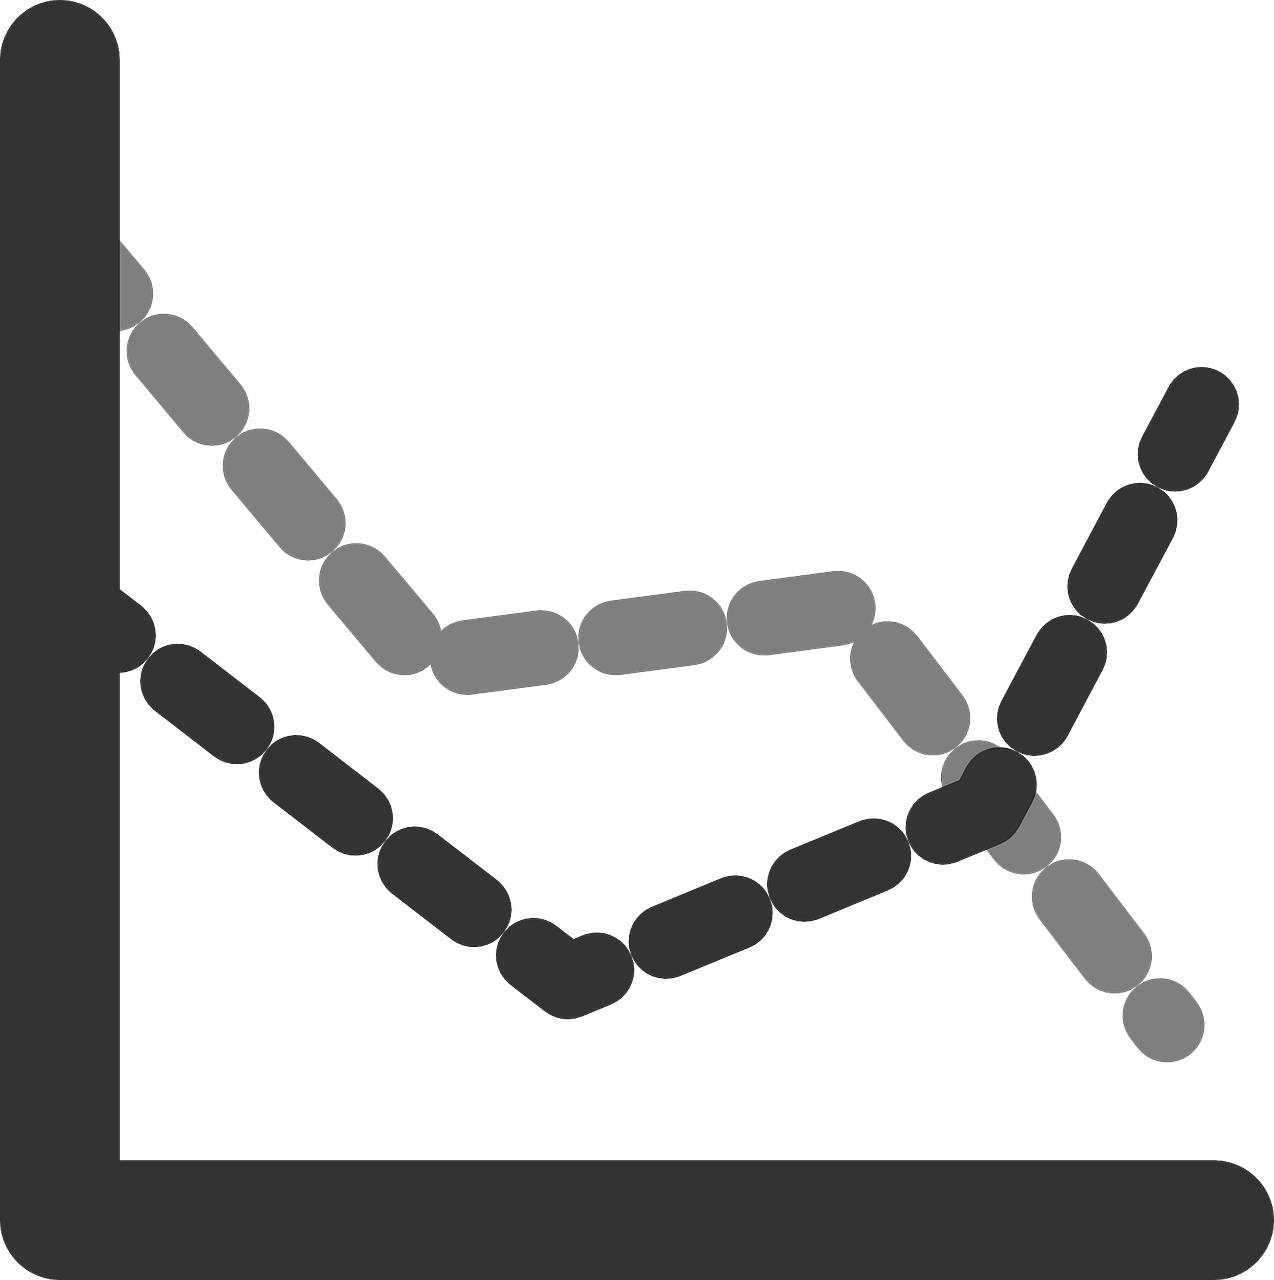
\includegraphics[height=1em]{BilderPräsentation/predict.png} Klassifikation und Vorhersage
				\end{tabular}
		}}
		
		\vspace{0.4em}
		
		\uncover<1->{
			\item[] 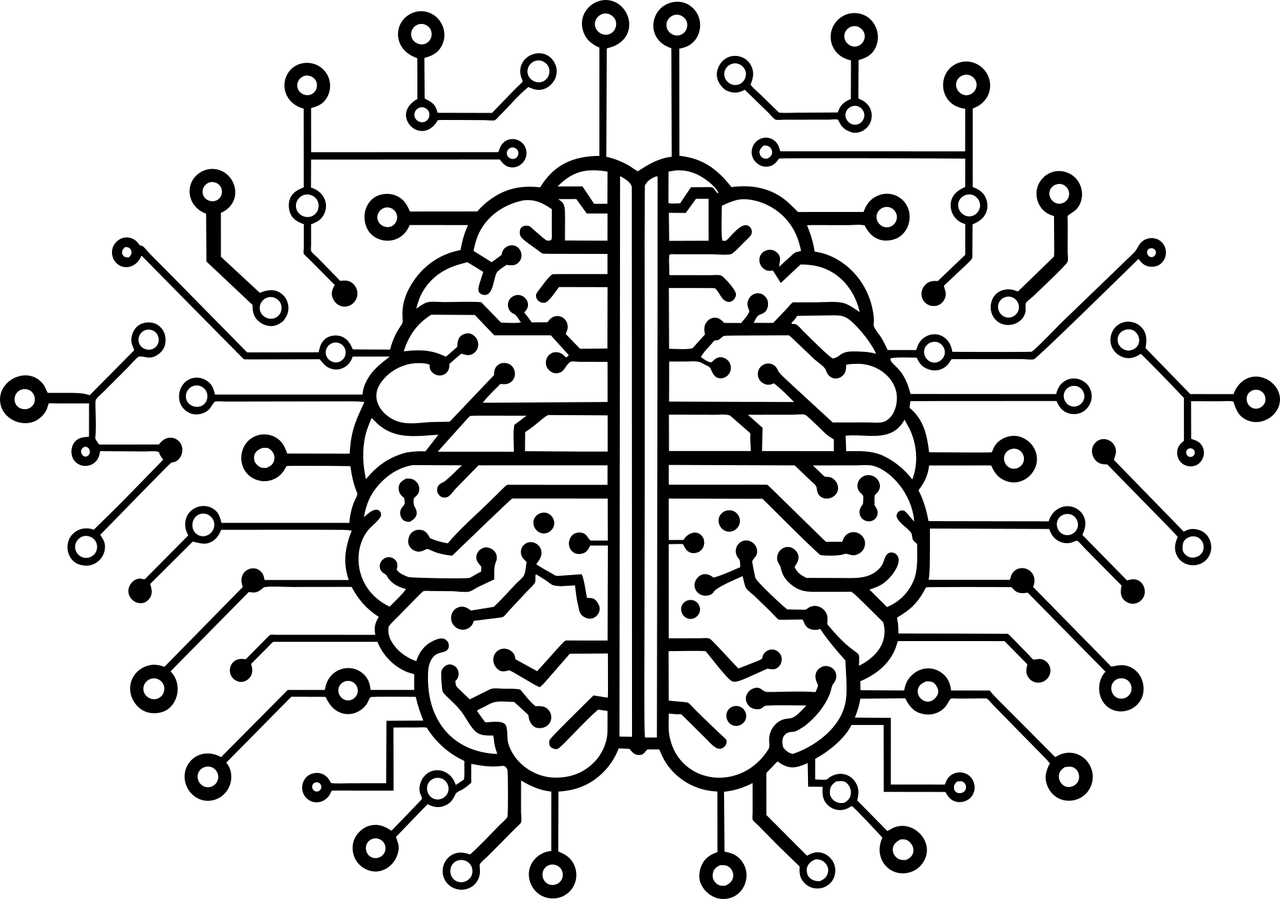
\includegraphics[height=1em]{BilderPräsentation/network.png} Sie lernen komplexe, nichtlineare Funktionen~\cite{antiga_deep_2020}}
		
		\vspace{0.4em}
		
		\uncover<2->{
			\item[] 
\includegraphics[height=1em]{BilderPräsentation/question.png} Wie ähnlich sind zwei Netze?
			\begin{itemize}
				\item Verständnis interner Repräsentationen
				\item Gleiche Architektur
				\item Unterschiedliches Training
		\end{itemize}}
		
	
		
	\end{itemize}
	{\tiny Quelle: Antiga et al., “Deep Learning with PyTorch”, Manning 2020~\cite{antiga_deep_2020}}
\end{frame}
\endgroup

\begingroup
\frametitle{Forschungsansatz}
\begin{frame}
\begin{itemize}
    \item \textbf{Ausgangspunkt}: Chan et al.~\cite{chan_affine_2024} schlagen einen Homotopie-basierten Ansatz zur Modellvergleichbarkeit vor:
    \begin{itemize}
      \item \textbf{Intrinsic Homotopy:} Wie gut kann eine Repräsentation in eine andere transformiert werden?
      \item \textbf{Extrinsic Homotopy:} Wie ähnlich ist das Modellverhalten bei gleichem Downstream-Task?
    \end{itemize}
    
    \vspace{0.8em}
    \item \textbf{Limitation}: Nur \emph{affine} Transformationen $\Rightarrow$ begrenzte Ausdruckskraft für komplexe Modelle.
    \end{itemize}
\vfill
{\tiny Quelle: Chan et al., “On Affine Homotopy between Language Encoders”, NeurIPS 2024~\cite{chan_affine_2024}}
\end{frame}
\endgroup

\begingroup
\frametitle{Forschungsfragen}
\begin{frame}
\vspace{0.8em}
\textbf{Forschungsfragen:}
\begin{itemize}
  \item Wie lassen sich intrinsic und extrinsic Homotopy im nichtlinearen Fall definieren?
  \item Erfassen nichtlineare Transformationen Ähnlichkeit besser als lineare?
  \item Besteht ein konsistenter Zusammenhang zwischen intrinsic und extrinsic Homotopy?
\end{itemize}
\end{frame}
\endgroup


\section{Neuronale Netze}
\frame{\tableofcontents[currentsection]}
\begingroup
\frametitle{Wie funktionieren neuronale Netze in der Praxis?}
\begin{frame}[plain]
	\vfill
	\begin{minipage}[c]{0.53\linewidth}
		\begin{itemize}
			\item Datengesteuerte, nichtlineare Funktionsapproximation
			\item Aufbau aus Layern \( f_1, f_2, \dots, f_L \)
			\item Architektur als Komposition:
			\[
			g(x) = f_L \circ f_{L-1} \circ \dots \circ f_1(x)
			\]
		\end{itemize}
	\end{minipage}
	\hfill
	\begin{minipage}[c]{0.44\linewidth}
		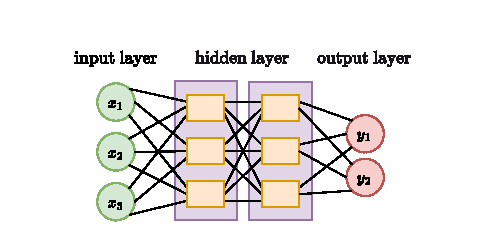
\includegraphics[width=0.95\linewidth]{BilderPräsentation/NN_ausgerichtet.drawio.pdf}
		\begin{itemize}\item []	{\scriptsize Schematische Darstellung eines neuronalen Netzwerks: Eingabe \(x_1, x_2, x_3\) wird durch eine Sequenz nichtlinearer Layer in Ausgaben \(y_1, y_2\) transformiert.} \end{itemize}
		
	\end{minipage}
	\vfill
\end{frame}
\endgroup


\begingroup
\frametitle{ Neuronale Netze: Black Box?}
\begin{frame}[plain]
	\centering
	
	\uncover<1->{	\begin{tikzpicture}[scale=1, every node/.style={font=\small}]
			% Input Text
			\node at (-5.5, 2) {Input $x \in \mathbb{R}^n$};
			
			% Pfeil von Input zum Hut
			\draw[very thick, ->] (-3,2) -- (-1.8,2);
			
			% Magic Hat Image
			\node at (0, 2.6) {
\includegraphics[width=2.2cm]{BilderPräsentation/magic_hat.png}};
			\node at (0, 1.3) {\footnotesize Neural Network};
			
			% Pfeil von Hut zu Output
			\draw[very thick, ->] (1.4,2) -- (2.8,2);
			
			% Output Text
			\node at (5.2, 2) {Output $g(x)$};
	\end{tikzpicture}}
	
	\vspace{1.5em}
	\uncover<1->{	\textbf{Frage:} Können neuronale Netze wirklich jede Funktion lernen?}
	
\end{frame}
\endgroup

\begingroup
\frametitle{Universal Approximation Theorem}
\begin{frame}
	\vspace{-1.3em}
	\begin{minipage}[t]{0.3\linewidth}
		\centering
		\vspace{0.5em}
		
\includegraphics[width=2.3cm]{BilderPräsentation/magic_hat.png}\\[0.5em]
	\end{minipage}%
	\hfill
	\begin{minipage}[t]{0.7\linewidth}
		\begin{block}{Universal Approximation Theorem~\cite{cybenko:hal-03753170}}
			\small
			Für jede stetige Funktion \( g \in C([0,1]^n) \) und jedes \( \varepsilon > 0 \)
			existiert ein neuronales Netz \( f \) der Form
			\[
			f(x) = \sum_{j=1}^{m} w^{(2)}_j\, \sigma\big( x^\top w^{(1)}_j - b_j \big),
			\]
			sodass \( \|g - f\|_\infty < \varepsilon \).
		\end{block}
	\end{minipage}
	

	{\tiny Quelle: Cybenko, “Approximation by superpositions of a sigmoidal function”, \textit{Mathematics of Control, Signals and Systems}, 1989~\cite{cybenko:hal-03753170}}
	
\end{frame}
\endgroup




\section{Natural Language Processing}
\frame{\tableofcontents[currentsection]}
\begingroup
\frametitle{Definition: Language Encoder}

\begin{frame}
	\begin{block}{Language Encoder}
		\small
		Ein \textbf{Language Encoder} ist eine Abbildung
		\[
		h : \Sigma^* \rightarrow \mathbb{R}^D,
		\]
		die Texte \(x \in \Sigma^*\) aus einem Alphabet \(\Sigma\) auf Vektoren \(h(x)\) im Repräsentationsraum \(\mathbb{R}^D\) abbildet.
		
		\vspace{0.3em}
		Die Menge aller solcher Encoder ist \(\mathcal{E}_V := V^{\Sigma^*}\).
		
	\end{block}
\end{frame}

\endgroup


\begingroup
\frametitle{Sprachverarbeitung mit Encoder-Decoder-Modellen}
\begin{frame}
	\centering
	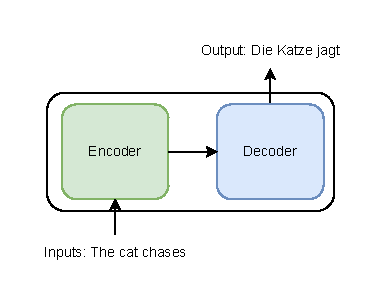
\includegraphics[width=0.4\linewidth]{BilderPräsentation/encoder_decoder.pdf}
	
	\begin{itemize}
		\item Encoder erzeugt eine Vektorrepräsentation aus dem Input-Text
		\item Decoder generiert daraus eine Zielsprache (z.\,B.\ Übersetzung)
		\item Modell lernt die Repräsentation durch Training auf großen Textdaten
	\end{itemize}
\end{frame}


\endgroup

\section{Ähnlichkeitsanalyse Neuronaler Netze}
\frame{\tableofcontents[currentsection]}
As mentioned in the introduction (see Section~\ref{Introduction}), understanding whether neural network models are similar is crucial in many areas of research and application.
This chapter is primarily based on the work by Klabunde et al.~\cite{klabunde_similarity_2024}, with additional references cited where appropriate.
Since there are various perspectives on what it means for models to be similar, we focus on two central and state-of-the-art viewpoints, illustrated in Figure~\ref{fig:SimilarityOfNN}. These are:
\begin{itemize}
    \item Representational similarity, and
    \item Functional similarity
\end{itemize}

We examine the key perspectives of \textit{representational similarity measures} and \textit{functional similarity measures} in more detail in Sections~\ref{RMS} and~\ref{FMS}, respectively.
%Similarity metrics have been widely studied, especially in relation to the invariance properties of neural networks~\cite{ding_grounding_2021, kornblith_similarity_2019}.



\begin{figure}[h]
    \centering
    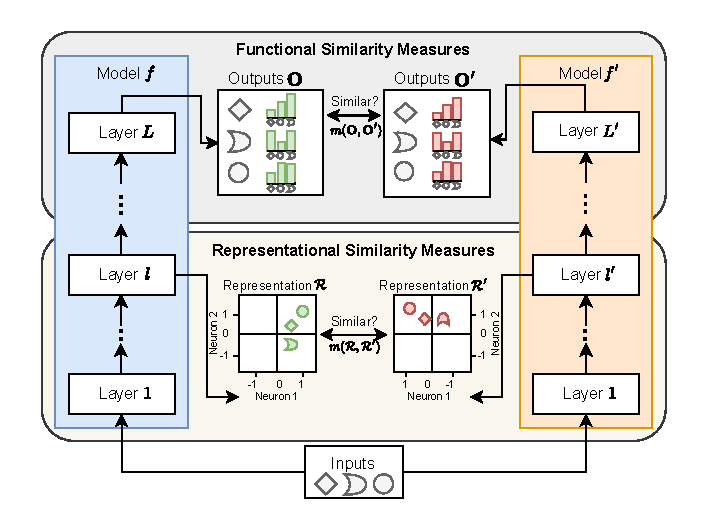
\includegraphics[width=\linewidth]{Abschlussarbeit/Pictures/Similarity90Deg.drawio.pdf}
    \caption{Visualization of representational and functional similarity \cite{klabunde_similarity_2024}.}
    \label{fig:SimilarityOfNN}
\end{figure}


\section{Intrinsic Homotopy}
\frame{\tableofcontents[currentsection]}
In Chapter~\ref{ISA}, we extended the concept of intrinsic homotopy to a family of non-linear models and transformations.  
In this context, we consider the distance map between two language encoders \( g, h \in \mathcal{E}_V \) defined in Definition ~\ref{eq:intrinsic_equation} as
\[
d_{\mathcal{F}_{\mathrm{Lip}_1}}(h, g) = \inf_{\psi \in \mathcal{F}_{\mathrm{Lip}_1}} \|h - \psi(g)\|_\infty,
\]
where \( \mathcal{F}_{\mathrm{Lip}_1} \subset \mathcal{C}_{V,W} \) denotes a subset of continuous functions, restricted in our case to non-linear neural networks.

Building on the theoretical considerations in Section~\ref{InrinsicHomotopyonNonlinTransf} and following the affine setting analyzed by Chan et al.~\cite{chan_affine_2024}, we constrain our analysis to \emph{non-linear 1-Lipschitz continuous neural networks}.  
This restriction ensures functional comparability and regularity of the learned transformations. The transformation \( \psi \in \mathcal{F}_{\mathrm{Lip}_1} \) is thus implemented as a neural network with architectural constraints that tries to enforce the Lipschitz property.

This setup allows us to compare encoder representations \( g(x) \) and \( h(x) \) by asking whether one can be mapped into the other in a structure-preserving way.  
If such a mapping exists in both directions (i.e., \( h \approx \psi(g) \) and \( g \approx \psi^{-1}(h) \)), we refer to \( g \) and \( h \) as \emph{exactly intrinsically affinely homotopic}.

Importantly, this notion of similarity is defined independently of any particular downstream task. Therefore, we analyze the final hidden layer representation of each language encoder, as it captures the model's abstract understanding before task-specific heads are applied.

\paragraph{Model Architecture.}
To estimate the intrinsic homotopy distance, we train transformation models that map representations from one encoder space into another. For each pair of encoders \( g \) and \( h \), we learn a mapping \( \psi \) such that
\[
\psi(g(x)) \approx h(x).
\]
We consider two types of transformation models:
\begin{itemize}
    \item a linear mapping (\texttt{LinearMap}), replicating the affine baseline from Chan et al.~\cite{chan_affine_2024} and
    \item a non-linear neural network (\texttt{NonLinearNetwork}) composed of fully-connected (dense) layers with ReLU activations. 
    Each layer is equipped with spectral normalization to ensure a controlled Lipschitz constant (i.e., \( \leq 1 \)).
\end{itemize}
This architectural flexibility enables controlled comparisons between linear and non-linear function classes under Lipschitz constraints.

\paragraph{Data Handling and Model Input.}
Each transformation model operates on precomputed hidden state representations \( g(x) \) and \( h(x) \), extracted from the final encoder layer for each input sample.  
These representations are stored on disk and loaded via \texttt{DataLoader} objects during training and evaluation.  
Training is supervised using the Huber loss.

\paragraph{Training Procedure.}
Models are trained using the Adam optimizer, as shown in Listing~\ref{lst:train-func} with early stopping based on validation loss.  
Training is performed on the same predefined training split that was previously used for extracting hidden representations, with the corresponding validation split used to monitor convergence.  
We explore multiple learning rates and record the corresponding loss trajectories.  
To ensure reproducibility across random seeds and tasks, all training runs are logged using process-specific log files.


\paragraph{Evaluation.}
As defined in Section~\ref{ISA}, the intrinsic homotopy distance is the infimum of the \( \ell^\infty \)-norm between \( h(x) \) and \( \psi(g(x)) \) over all admissible transformations \( \psi \in \mathcal{F}_{\mathrm{Lip}_1} \subset \mathcal{C}_{V,W} \).  
After training, the learned transformation \( \psi^* \) approximates this infimum within the class of nonlinear 1-Lipschitz neural networks.

To evaluate the quality of this approximation, we compute the maximum deviation between the transformed and target representations over a held-out test set:
\[
\max_{x \in \mathcal{D}_{\mathrm{test}}} \| h(x) - \psi^*(g(x)) \|_\infty.
\]
This value serves as a practical estimate of the intrinsic homotopy distance.

In addition, we compute the Pearson and Spearman correlation coefficient between the transformed and target representations over the test set.  
These metrics capture whether the transformation \( \psi^* \) preserves linear or monotonic structure between the input and output representations:
\begin{itemize}
	\item The \emph{Pearson correlation coefficient} measures the linear correlation between components of \( h(x) \) and \( \psi^*(g(x)) \).
	\item The \emph{Spearman rank correlation} captures the strength of any monotonic (not necessarily linear) relationship between the two vectors.
\end{itemize}
High correlation values indicate that \( \psi^* \) not only minimizes pointwise distances but also aligns structural trends in the representation space.

Formally, the \emph{Pearson correlation coefficient} between the target and predicted representations is defined as
\[
\rho_{\mathrm{Pearson}} = \frac{\operatorname{Cov}(h(x), \psi^*(g(x)))}{\sigma_{h(x)} \, \sigma_{\psi^*(g(x))}},
\]
where \( \operatorname{Cov}(\cdot, \cdot) \) denotes the empirical covariance and \( \sigma \) the standard deviation computed over the test set.

The \emph{Spearman rank correlation} is defined analogously, but computed on the rank-transformed data:
\[
\rho_{\mathrm{Spearman}} = \rho_{\mathrm{Pearson}}(\operatorname{rank}(h(x)), \operatorname{rank}(\psi^*(g(x)))).
\]



\begin{lstlisting}[language=Python, caption={Computation of $\|h(x) - \psi(g(x))\|_\infty$ in PyTorch}, label={lst:linf-computation}]
with torch.no_grad():
    for g_batch, h_batch in test_dataloader:
        output = model(g_batch)
        diff = h_batch - output
        dist = torch.max(torch.abs(diff)) # ||h - \psi(g)||_\infty
        all_dist.append(dist.item())
\end{lstlisting}

The maximum deviation across all batches is then used as an estimate for the distance:
\begin{lstlisting}[language=Python]
overall_max = max(all_dist)
\end{lstlisting}

This value corresponds to the right-hand side of Definition~\ref{eq:intrinsic_equation}, and serves as an empirical approximation to the intrinsic homotopy distance \( d_{\mathcal{F}_{\mathrm{Lip}_1}}(g, h) \).

In addition, we compute the following metrics to enable a quantitative comparison between linear and non-linear transformations (see Section~\ref{exp:IntrinsicHOm} for detailed analysis):

\begin{itemize}
    \item the Spearman rank correlation between predicted and target representations,
    \item the Pearson correlation between input and output representations (averaged over all features),
    \item an upper bound on the Lipschitz constant via the product of spectral norms of the network's weight matrices,
    %\item a lower bound estimate using Monte Carlo sampling of Jacobians on random Gaussian input vectors.
\end{itemize}

All hyperparameters, including learning rate, number of epochs, batch size, and network type, are configurable via command-line arguments. 
Results are stored in structured directories, and summary metrics are exported in JSON format for subsequent analysis.

\section{Implementierung und Experimente}
\frame{\tableofcontents[currentsection]}
\begingroup
\frametitle{Implementierung: Trainingsprozedur (nichtlinear)}
\begin{frame}
	\footnotesize
	\begin{itemize}
		\item \textbf{Ziel:} Lerne eine Transformation \( \psi \), sodass \( \psi(g(x)) \approx h(x) \) für Encoderrepräsentationen \( g, h \)
		\item \textbf{Modellklassen:}
		\begin{itemize}
			\item \texttt{LinearMap} (affine Projektion)
			\item \texttt{NonLinearNetwork} (1-Lipschitz-MLP via Spektralnorm)
		\end{itemize}
		\item \textbf{Evaluation:}
		\begin{itemize}
			\item \( \max\limits_{x \in \mathcal{D}_{\text{test}}} \| h(x) - \psi(g(x)) \|_\infty \)
			\item Pearson-/Spearman-Korrelation, Lipschitz-Konstante
		\end{itemize}
	\end{itemize}
	
\end{frame}
\endgroup

%\begingroup
%\frametitle{Train Nonlinear Network}
%\begin{frame}[fragile]
%	\begin{figure}
%		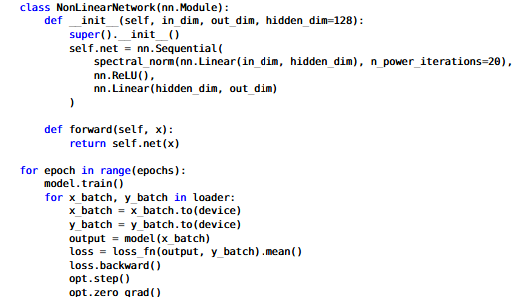
\includegraphics[width=0.8\linewidth]{BilderPräsentation/TrainNN.png}
%	\end{figure}
%\end{frame}
%\endgroup 

\begingroup
\frametitle{Reproduktion der Intrinsic Homotopy Werte}
\begin{frame}{Reproduktion der Intrinsic Homotopy Werte}
	\begin{columns}
	\column{0.4\textwidth}
	\begin{minipage}[t]{\linewidth}
		\vspace{1em}
		\begin{itemize}
			\tiny
			\uncover<1->{\item  Ziel: Reproduktion der Distanzwerte aus Chan et al.~\cite{chan_affine_2024}}
			\uncover<2->{\item Erster Versuch: Approximation der Werte im Testsplit, selber Architektur und $\max(\text{loss})$}
			\uncover<3->{\item Zweiter Versuch: Approximation der Werte mit im Trainingssplit, selber Architektur und $\max(\text{loss})$}
			\uncover<4->{\item Modelle sind aufgrund des Trainings auf den Trainingsdaten gebiased, daher erfolgen Tests auf einem separaten Testsplit}
		\end{itemize}
	\end{minipage}
	\column{0.6\textwidth}
\uncover<1->{	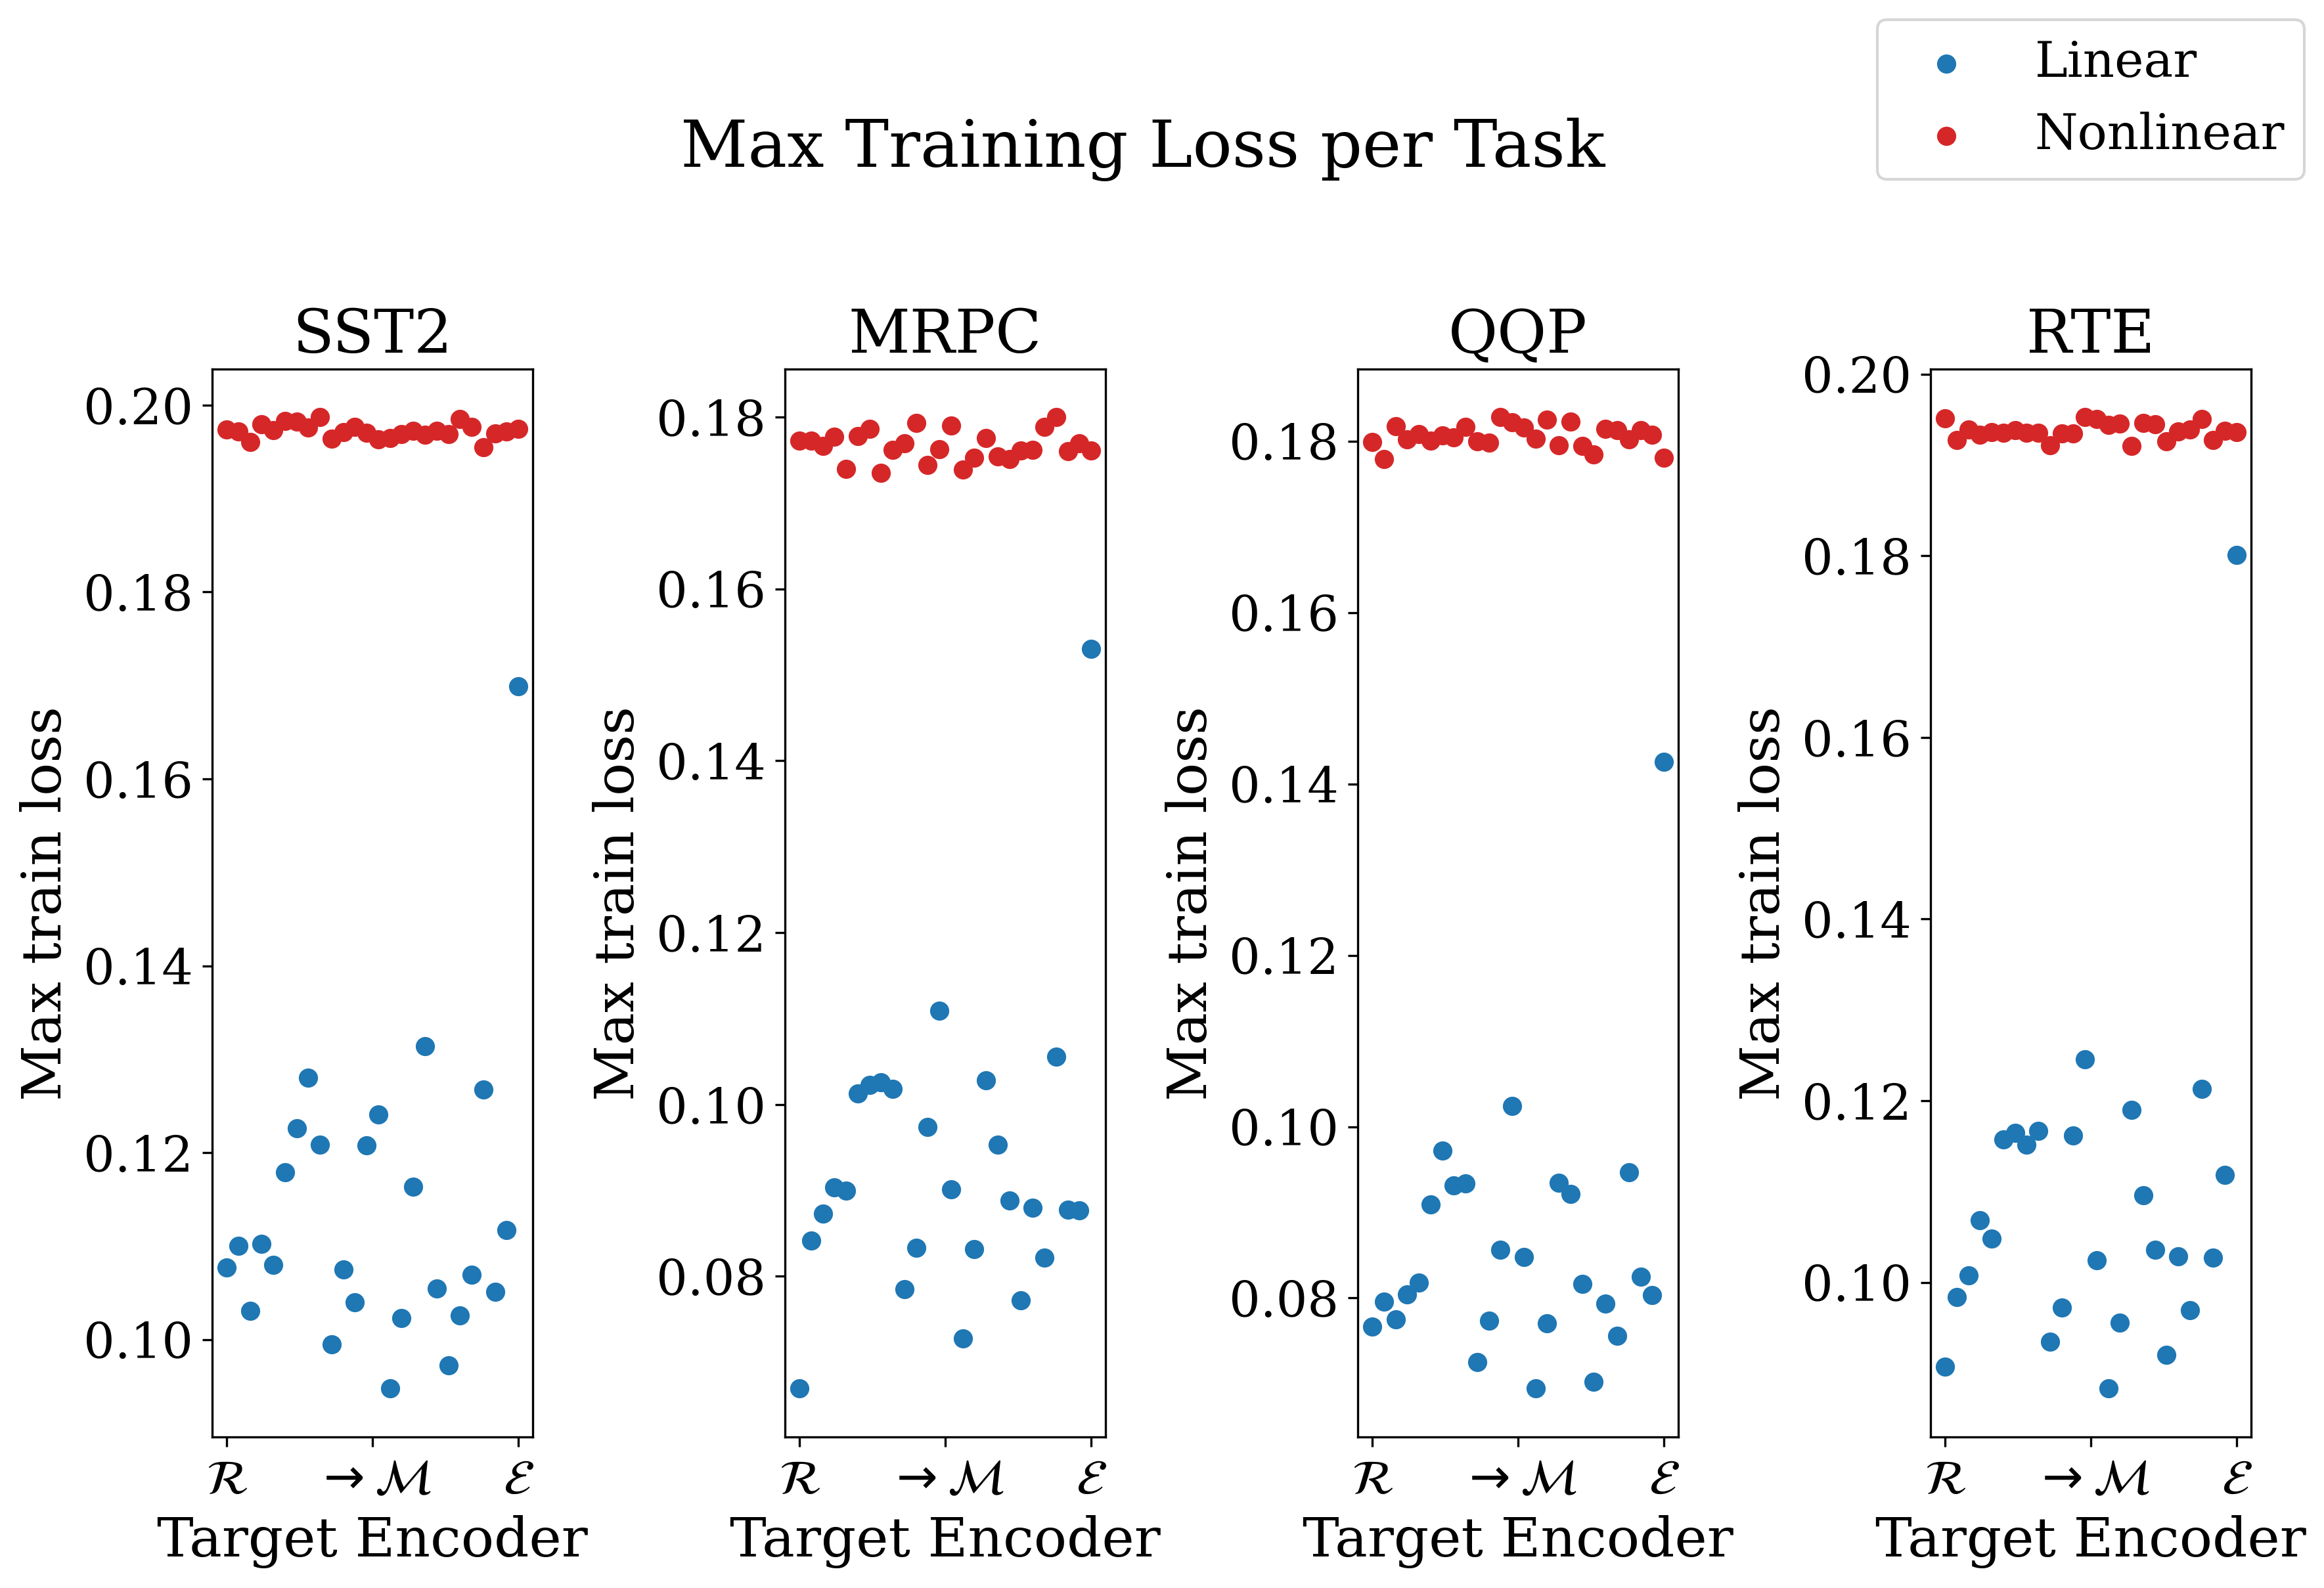
\includegraphics[width=\linewidth]{BilderPräsentation/New_all_in_one_scatter_praes.png}}
\end{columns}
\end{frame}
\endgroup


\begingroup
\frametitle{Experiment: Intrinsic Homotopy}
\begin{frame}
	\begin{columns}
		\column{0.4\textwidth}
		\begin{minipage}[t]{\linewidth}
			\vspace{1em}
			\tiny
			\begin{itemize}
				\tiny
				\uncover<1->{\item Analyse linearer und nicht-linearer Transformationen}
			\end{itemize}
		\end{minipage}
		
		\column{0.6\textwidth}
		\uncover<2->{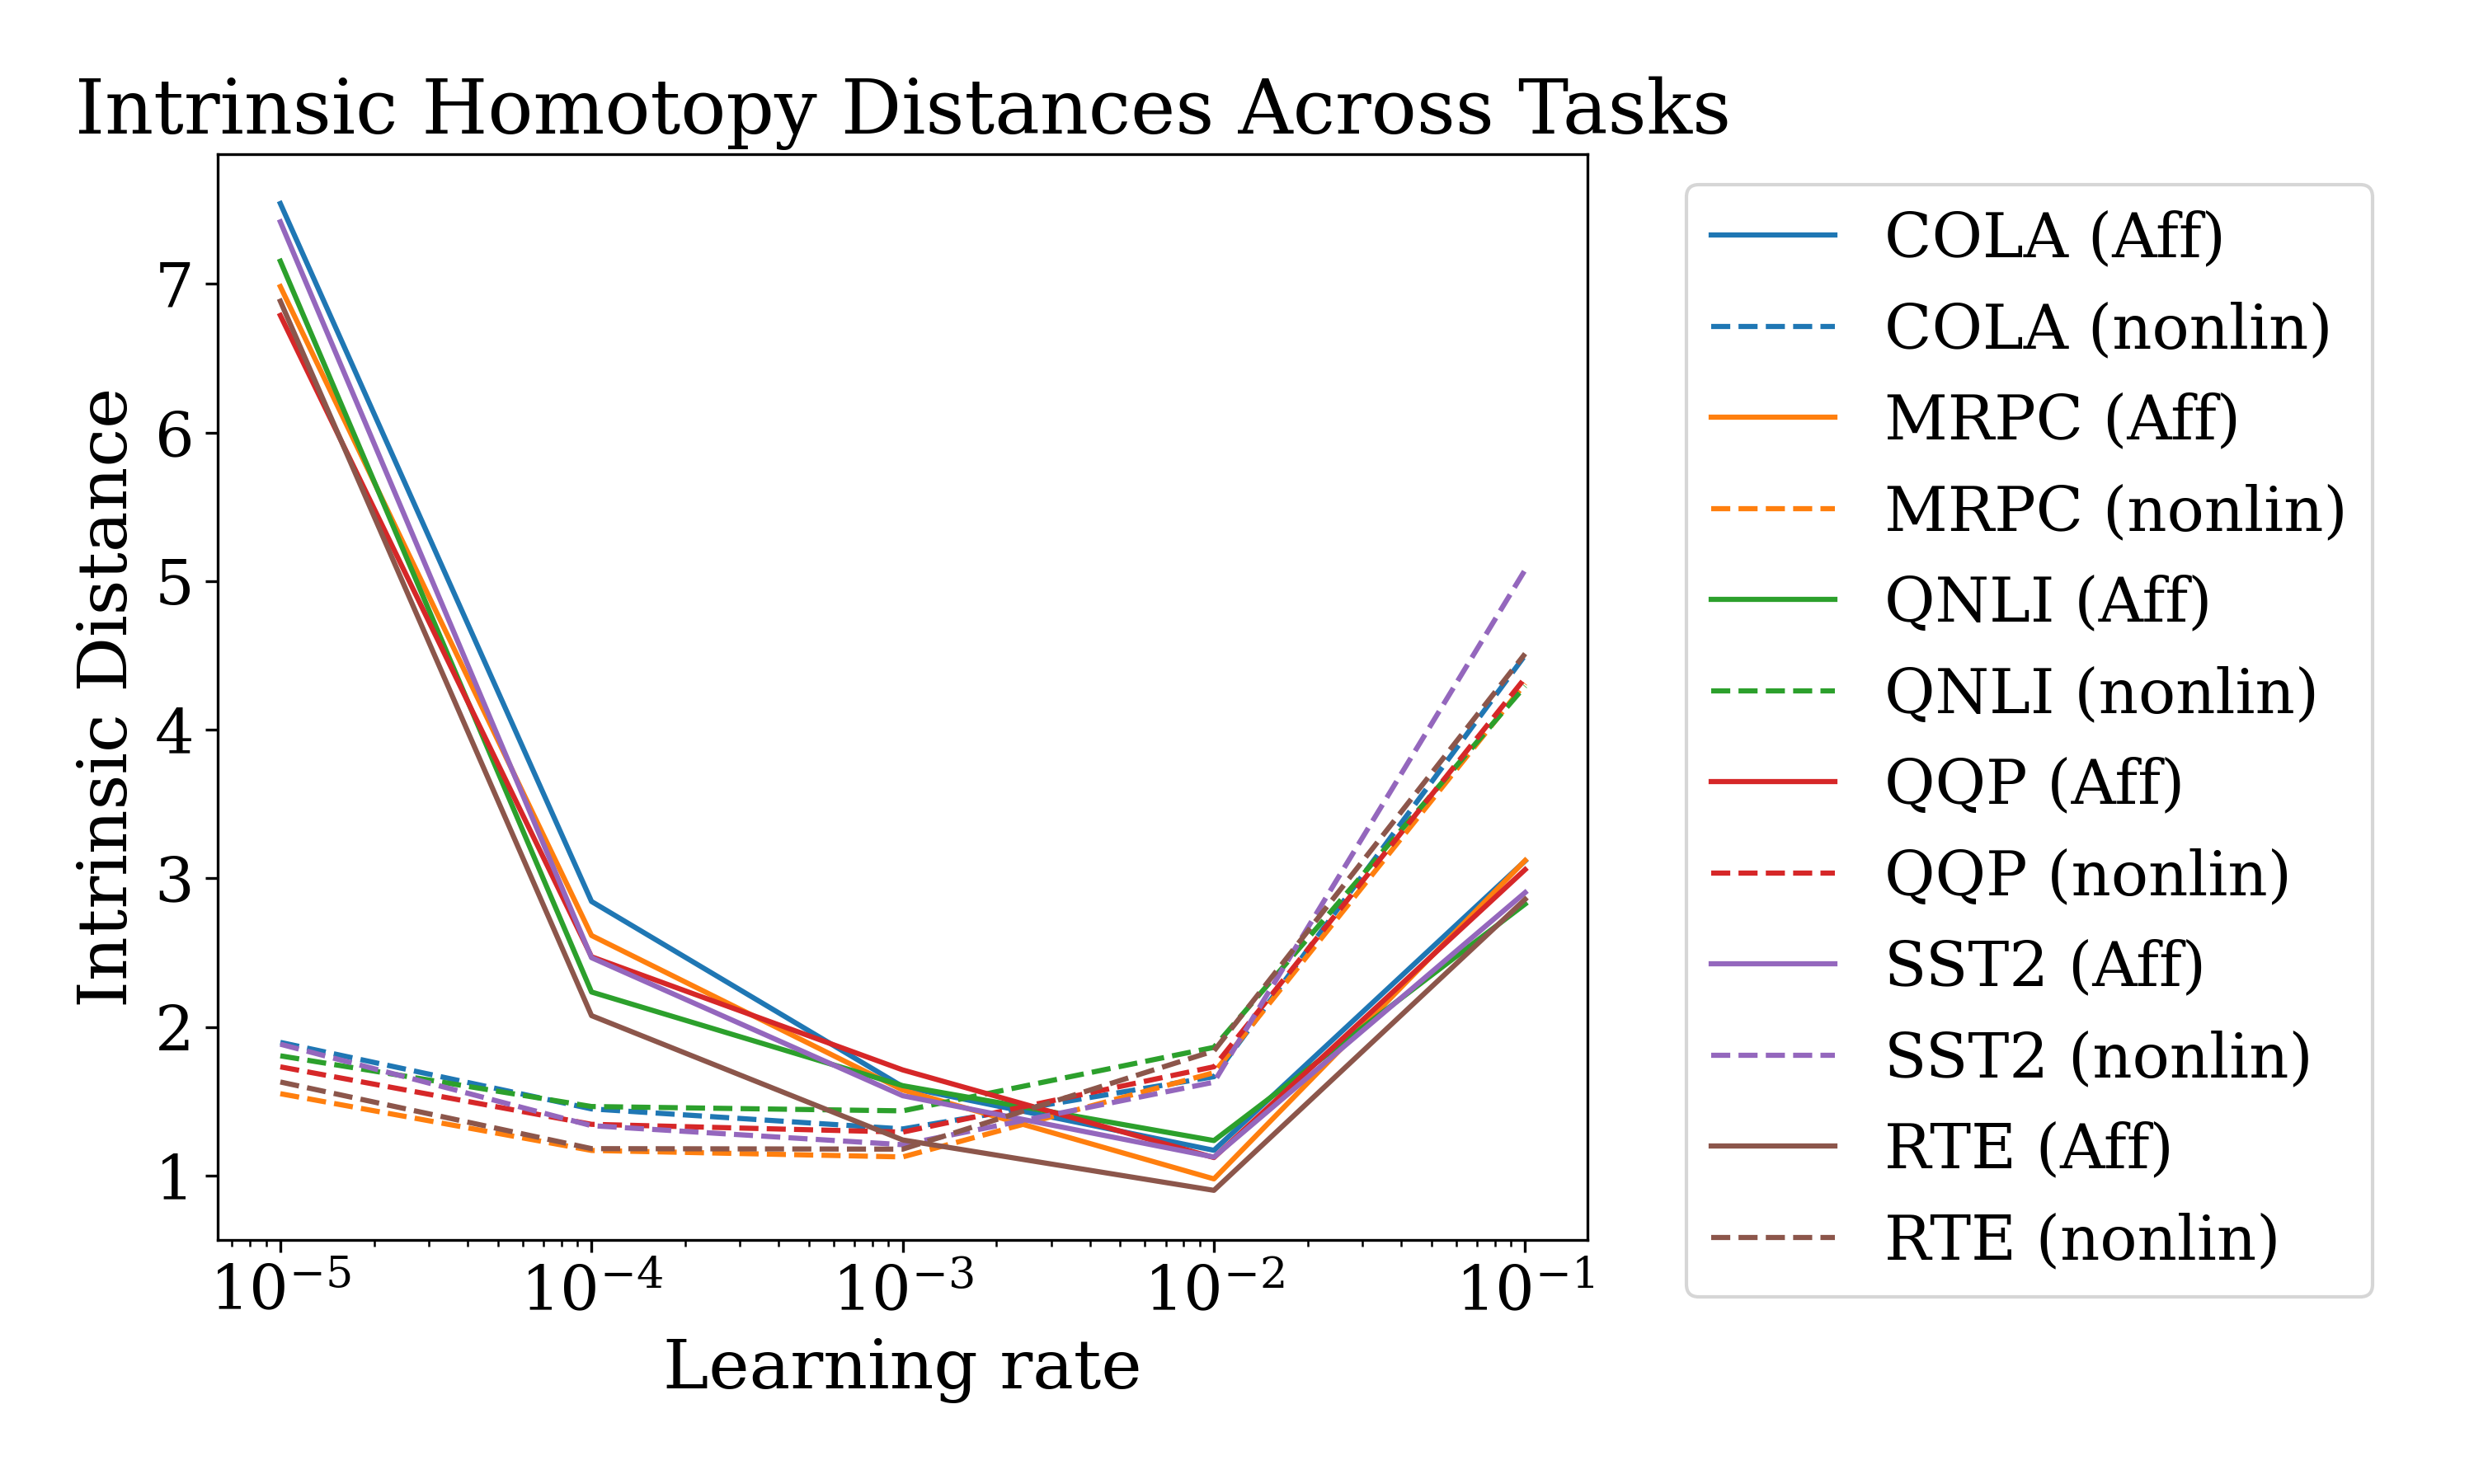
\includegraphics[width=1.1\linewidth]{BilderPräsentation/intrinsic_distance_all_tasksPräsi.png}}
	\end{columns}
\end{frame}
\endgroup

\begingroup
\frametitle{Experiment: Intrinsic Homotopy}
\begin{frame}
			\vspace{1em}
			\tiny
			\begin{itemize}
				\tiny
				\uncover<1->{\item Analyse linearer und nicht-linearer Transformationen}
				\uncover<2->{\item Pearson-Koeffizient: zeigt linearen Zusammenhang zwischen Input und Output}
				\uncover<3->{\item Kaum linearer Zusammenhang $\Longrightarrow$ schwierig, lineare Transformation zu finden}
				\uncover<4->{\item Lineare Modelle reichen nicht aus, um Strukturähnlichkeit realistisch abzubilden}
			\end{itemize}
		\begin{table}[H]
			\centering
			\caption{Pearson Correlation Score \(r\) across tasks and learning rates.}
			\label{tab:correlation-transposed}
			\begin{tabular}{l c ccccccc}
				\toprule
				 & \texttt{QNLI} & \texttt{CoLA} & \texttt{MRPC} & \texttt{QQP} & \texttt{RTE} & \texttt{SST-2} \\
				\midrule
				\(r\) 
				&  \(5\cdot10^{-6}\) & \(4\cdot10^{-6}\) & \(4\cdot10^{-6}\) & \(5\cdot10^{-6}\) & \(3\cdot10^{-6}\) & \(5\cdot10^{-6}\)
			\end{tabular}
		\end{table}
\end{frame}
\endgroup




\begingroup
\frametitle{Experiment: Intrinsic Homotopy}
\begin{frame}
	\begin{columns}
		\column{0.4\textwidth}
		\begin{minipage}[t]{\linewidth}
			\vspace{1em}
			\tiny
			\begin{itemize}
				\tiny
				\uncover<1->{\item \textbf{Beispiel-Task:} \textbf{MRPC} – geringste Distanzen im Intrinsic-Vergleich}
				\uncover<2->{\item \textbf{Heatmaps:} Modelle mit $d_{\mathcal{C}}(h, g) < 1$  und  $d_{\mathcal{C}}(g, h) < 1$ gelten als \emph{homotop} (weiß markiert)}
				\uncover<3->{\item \textbf{Beobachtungen:}}
				\begin{itemize}
					\tiny
					\uncover<4->{\item Deutlich mehr homotope Modellpaare bei \textbf{nichtlinearen Transformationen}}
					\uncover<5->{\item Besonders bei kleinen Lernraten (\texttt{lr} = $10^{-5}$ bis $10^{-3}$)}
					\uncover<6->{\item Höhere Lernraten $\Rightarrow$ instabileres Training, weniger Struktur}
				\end{itemize}
			\end{itemize}
		\end{minipage}
		
		\column{0.6\textwidth}
		\uncover<2->{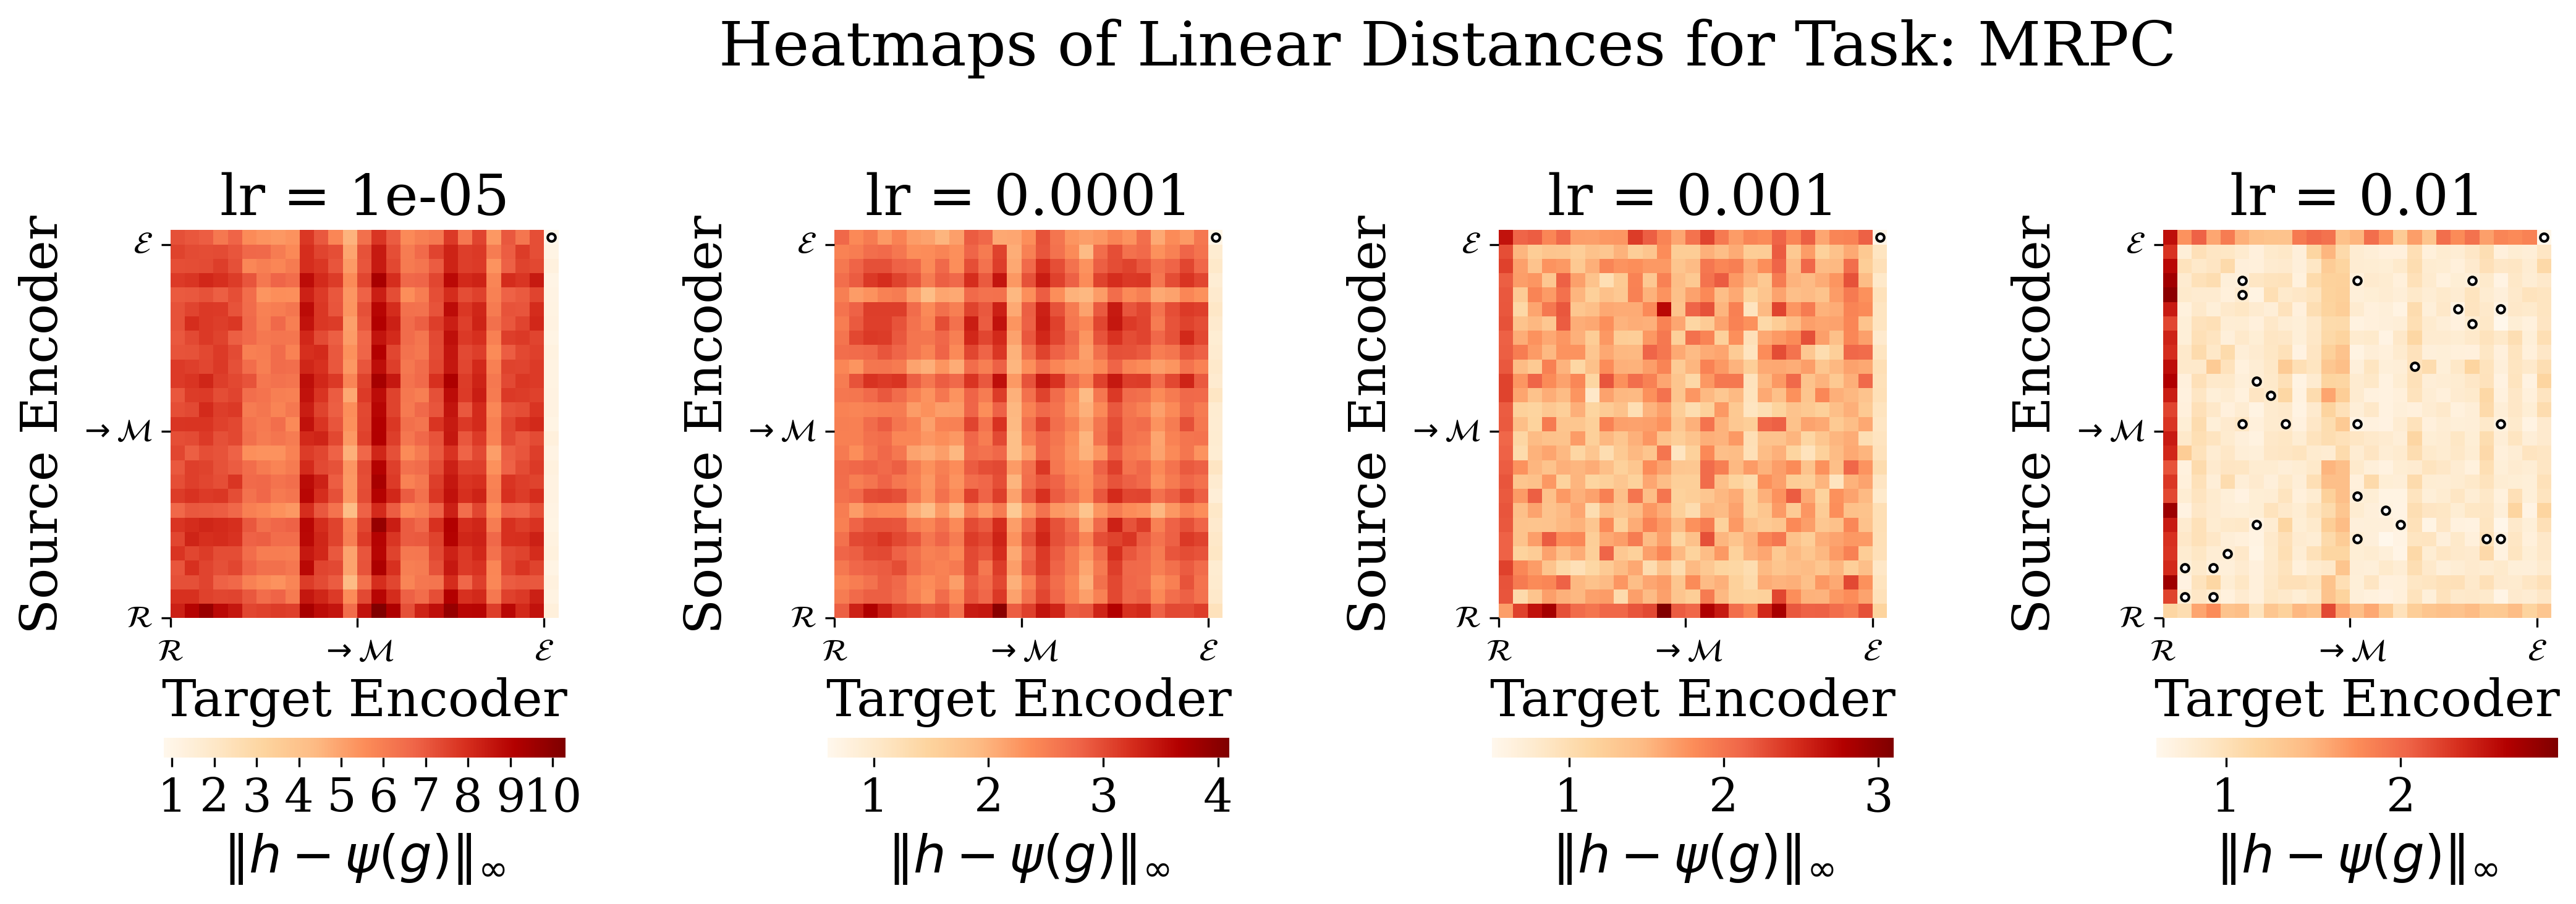
\includegraphics[width=\linewidth]{BilderPräsentation/PräsiHeatmap_linear_distance_all_lrs_mrpc_homotopy.png}\\[1ex]}
		\uncover<2->{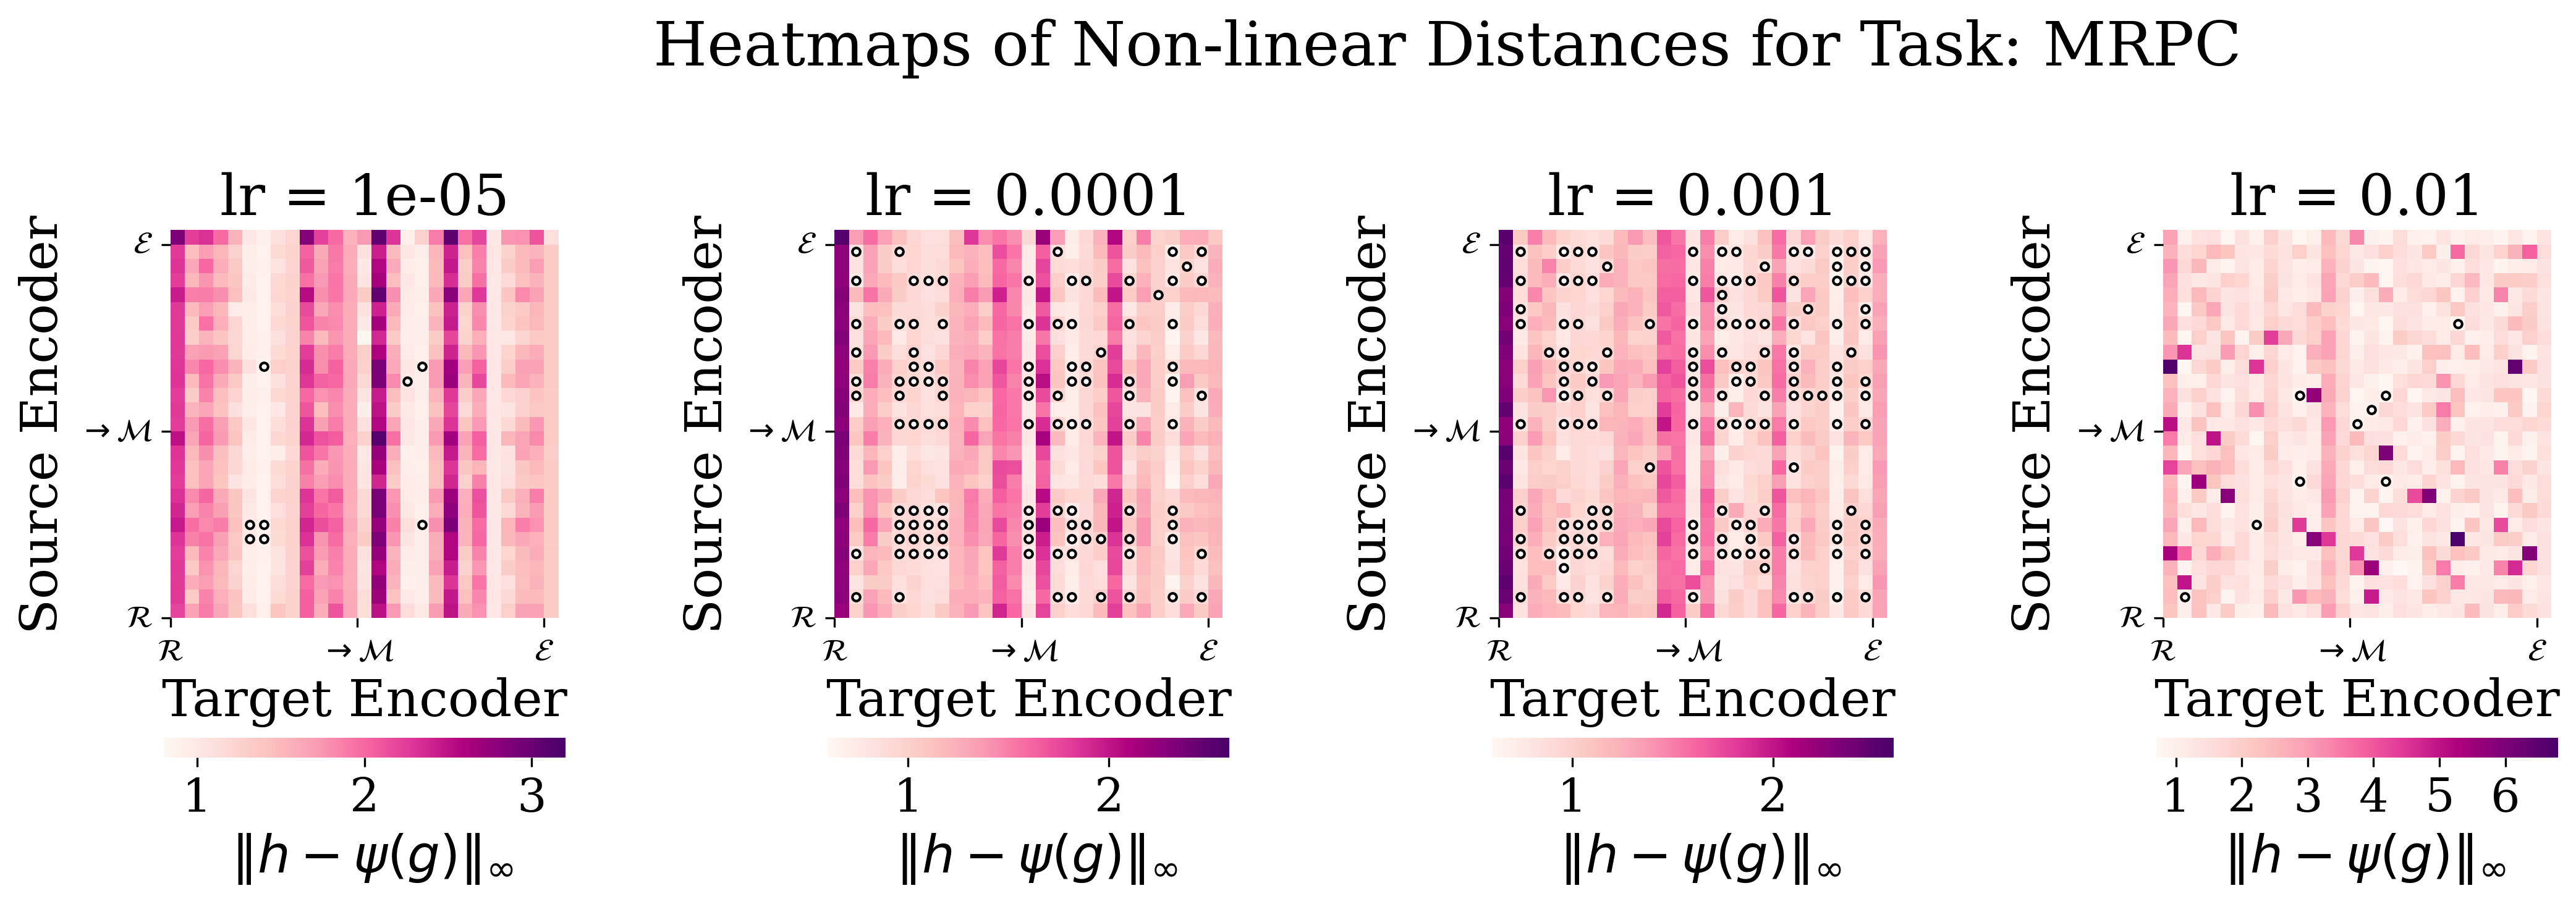
\includegraphics[width=\linewidth]{BilderPräsentation/PräsiHeatmap_nonlinear_distance_all_lrs_mrpc_homotopy.png}}
	\end{columns}
\end{frame}
\endgroup


\begingroup
\frametitle{Experiment: Intrinsic vs Extrinsic Homotopy}
\begin{frame}
	\tiny
	\begin{itemize}
		\tiny
		\uncover<1->{\item Intrinsic $\Rightarrow$ Extrinsic in Chan et al.~\cite{chan_affine_2024}} 
		\uncover<2->{\item \textbf{Beobachtungen:}}
		\begin{itemize}
			\tiny
			\uncover<2->{\item Beste Übereinstimmung bei \textbf{QNLI} (höchste Regressionsgüte)}
			\uncover<2->{\item Aber selbst hier nur leichter zusammenhang }
		\end{itemize}
	\end{itemize}
	\vspace{1em}
	\uncover<2->{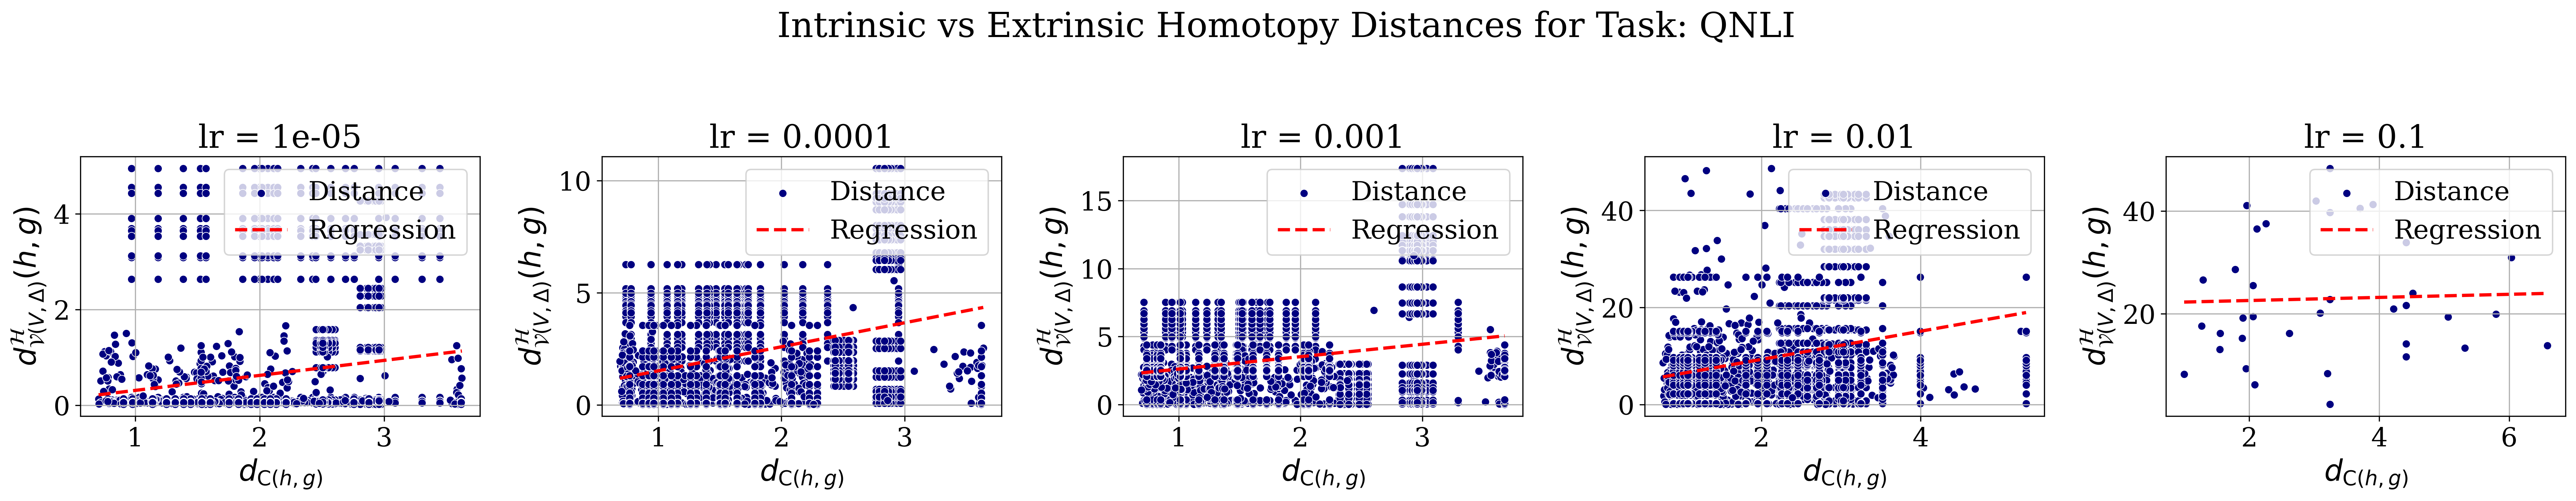
\includegraphics[width=1\linewidth]{BilderPräsentation/intrinsicVSextrinsic/PräsiDist_extr_intr_subplots_qnli.png}}
\end{frame}
\endgroup

\begingroup
\frametitle{Experiment: Intrinsic vs Extrinsic Homotopy}
\begin{frame}
	\tiny
	\begin{itemize}
		\tiny
		\uncover<1->{\item \textbf{Beobachtungen:}}
		\begin{itemize}
			\tiny
			\uncover<1->{\item Regressionslinie bei \textbf{MRPC} nahezu parallel zur X-Achse }
			\uncover<1->{\item $\Rightarrow$ Kaum Zusammenhang zwischen intrinsischer und extrinsischer Ähnlichkeit in unserem Setup, stark vom Task abhängig}
		\end{itemize}
	\end{itemize}
	\vspace{1em}
		\uncover<1->{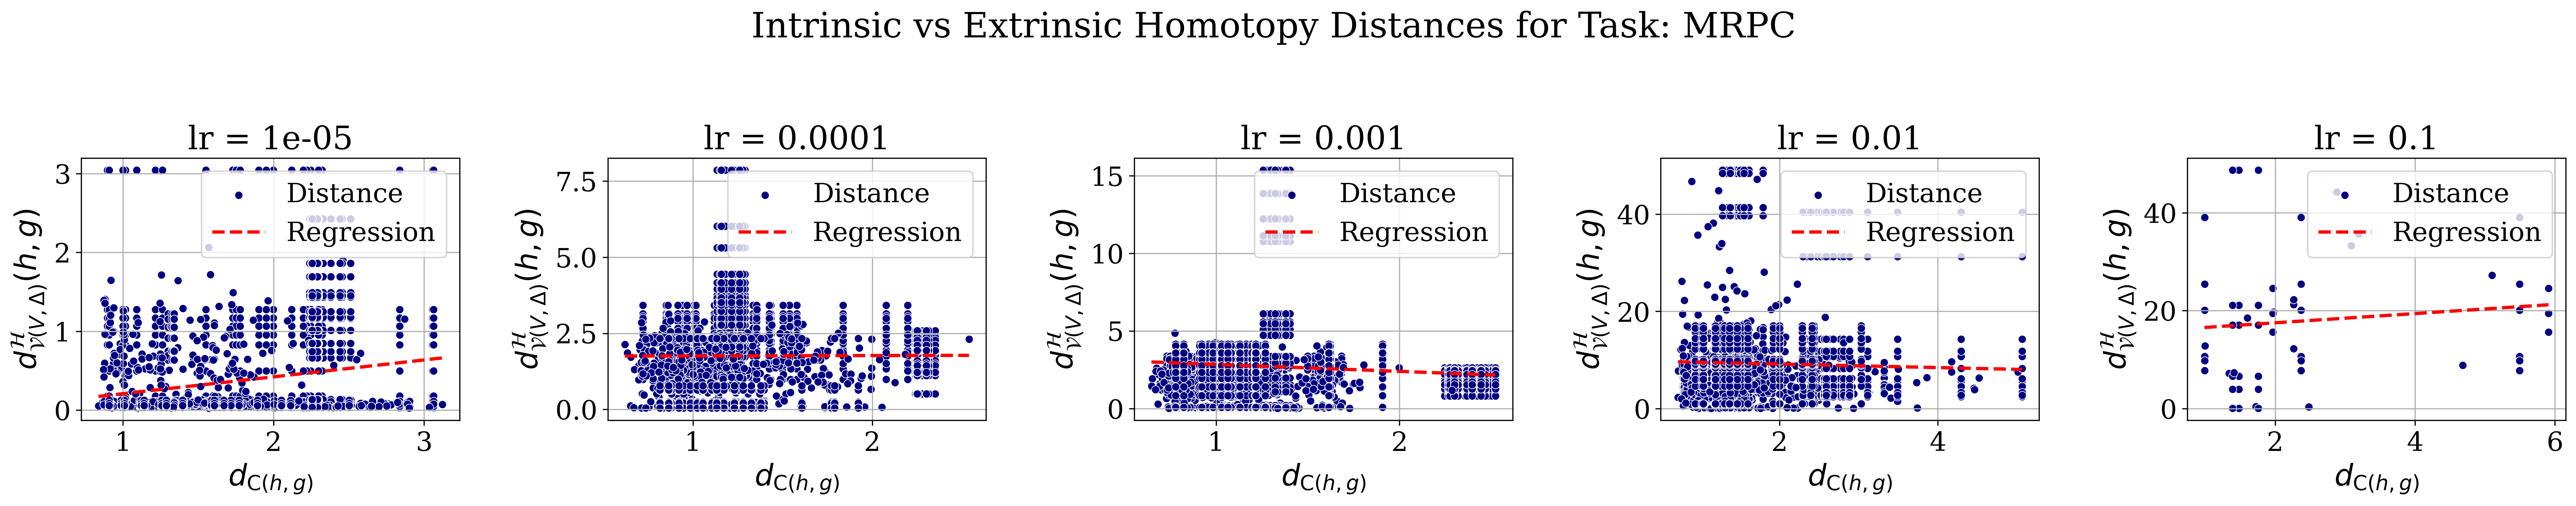
\includegraphics[width=1\linewidth]{BilderPräsentation/intrinsicVSextrinsic/PräsiDist_extr_intr_subplots_mrpc.png}}
\end{frame}
\endgroup


\section{Zusammenfassung und Future Work}
\frame{\tableofcontents[currentsection,currentsubsection]}
\begingroup
\frametitle{Fazit}
\begin{frame}
	\begin{itemize}
		\setlength\itemsep{0.6em}
		\uncover<1->{\item Nichtlineare Homotopie erlaubt tiefere Vergleiche von Sprachmodellen als affine Baselines.}
		\uncover<2->{\item Besonders bei kleinen Lernraten entstehen dichte, homotope Strukturen zwischen Encodern.}
		\uncover<3->{\item Zusammenhang zwischen intrinsischer und extrinsischer Homotopie ist stark \textbf{task-abhängig} (z.\,B. QNLI vs. SST-2).}
	\end{itemize}
\end{frame}
\endgroup

\begingroup
\frametitle{Ausblick}
\begin{frame}
	\begin{itemize}
		\setlength\itemsep{0.9em}
		\uncover<1->{\item \textbf{Modellvielfalt:} Erweiterung auf andere Modellarten.}
		\uncover<2->{\item \textbf{IT-Sicherheit:} Anwendung im Bereich Poisoning- oder Backdoor-Angriffe.}


	\end{itemize}
\end{frame}
\endgroup



\appendix\nocite{*}
\section{Literatur}
\begin{frame}[allowframebreaks, nosection]
	\frametitle{Literatur}
	\bibliography{quellen}

\end{frame}

\begin{frame}[nosection]
    Vielen Dank für Ihre Aufmerksamkeit!
\end{frame}


\end{document}